\section{Analyse de marché}

\subsection{Win-posturo}


WIN-POSTURE NV Software est une plateforme d'analyse en posturographie statique. 
Elle se distingue par sa convivialité et son ergonomie, facilitant son utilisation. 
Il offre la possibilité de créer et de gérer des protocoles d'acquisition tout en permettant de paramétrer des normes conformes aux recommandations de l'AFP85 (SOFPEL). 
Ce logiciel intègre des fonctionnalités avancées telles que l'analyse fractale et l'analyse par ondelette. 
Il permet également de comparer les résultats des examens pour chaque patient, avec des données facilement exportables vers Excel. 
Les rapports et bilans générés sont entièrement personnalisables, et le logiciel propose des outils intégrés pour la création de courriers et le publipostage.


WIN-POSTURE NV Software une nouvelle plateforme d’analyse de stabilographie statique qui a comme fonctionnalités : 
\begin{itemize}
    \item \textbf Convivialité et ergonomie incomparables.
    \item \textbf Création et gestion des protocoles d’acquisition
    \item \textbf Paramétrage des normes et référentiels 
    \item \textbf Production de la totalité des données stabilométriques normalisées APE 85
    \item \textbf Nouvelles fonctionnalités issues de l’actualité scientifique (option : ondelettes, analyses fractales et de diffusion…) 
    \item \textbf Possibilité de comparaison des examens 
    \item \textbf Multiples Visualisations du signal stabilométrique 
    \item \textbf Edition de rapports et bilans personnalisables  
    \item \textbf Exportation directe des données stabilométriques vers Excel 
    \item \textbf Editeur de courrier 
    \item \textbf publipostage
\end{itemize}

\begin{figure}[H]
    \centering
    \begin{subfigure}[b]{0.45\textwidth}
      \centering
      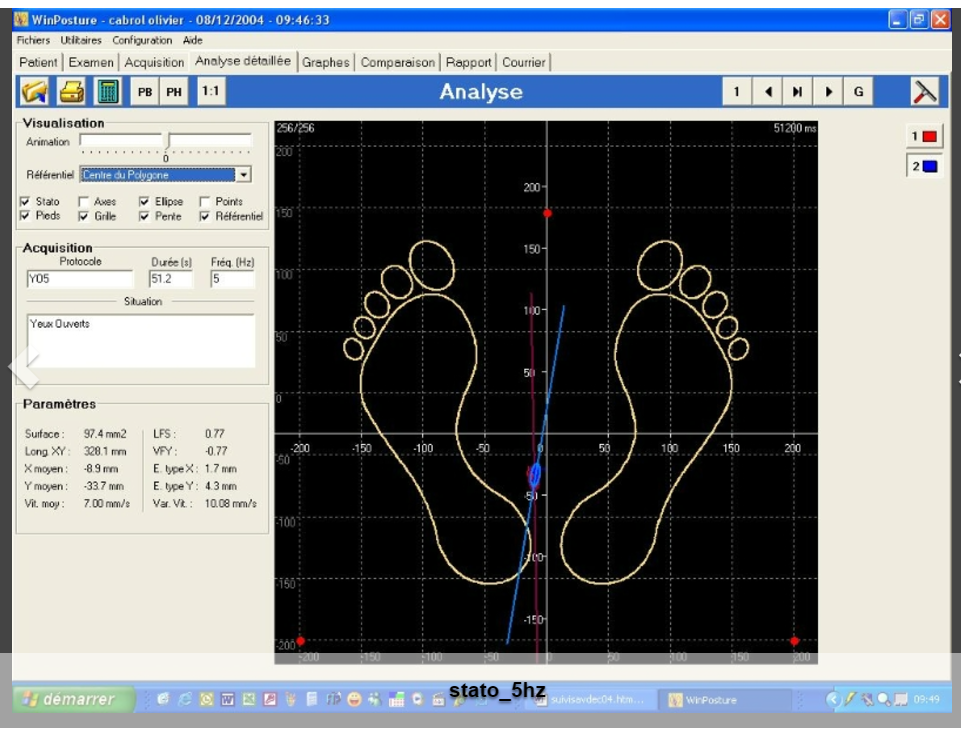
\includegraphics[height=5cm]{images/pression_plantaire/winposture.png}
      \caption{Logiciel Winposture}\label{fig:winposture}
    \end{subfigure}
    \begin{subfigure}[b]{0.5\textwidth}
        \centering
        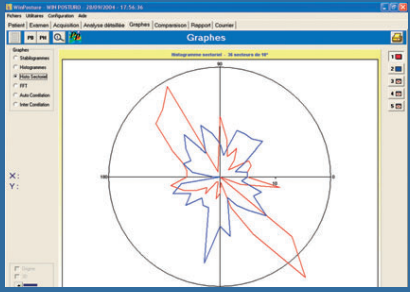
\includegraphics[height=5cm]{images/analyse_marche/winposture_ellipse.png}
        \caption{Visualisation de l'ellipse de confiance}\label{fig:winposture_ellipse_de_confiance}
    \end{subfigure}
    \begin{subfigure}[b]{0.5\textwidth}
        \centering
        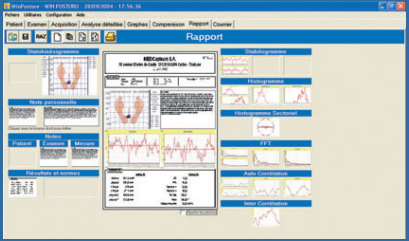
\includegraphics[height=5cm]{images/analyse_marche/winposture_rapport.png}
        \caption{Rapport du logiciel sur un cas patient}\label{fig:winposture_rapport}
    \end{subfigure}
    \begin{subfigure}[b]{0.5\textwidth}
        \centering
        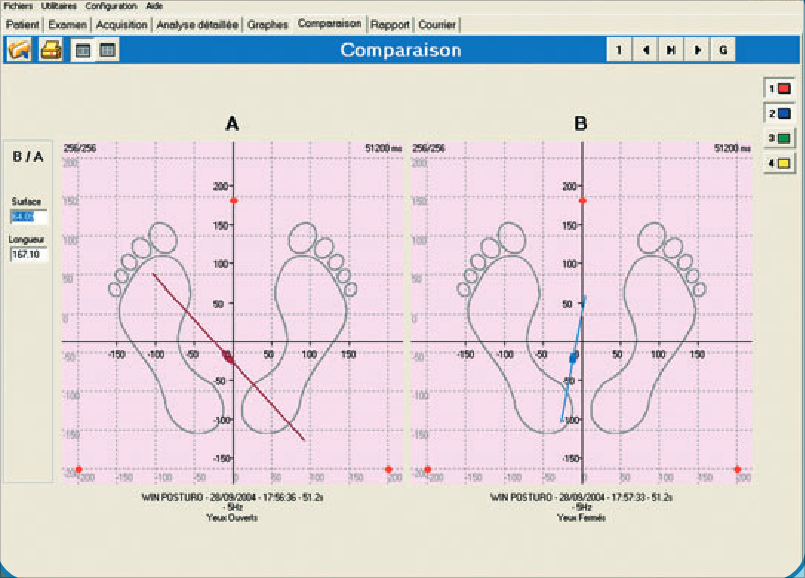
\includegraphics[height=5cm]{images/analyse_marche/comparaison_yo_yf.png}
        \caption{Comparaison de l'équilibre orthostatique yeux ouverts/fermés}\label{fig:winposture_comparaison_yo_yf}
    \end{subfigure}
\end{figure}

\subsection{Fusyo}

Fusyo combine analyses stabilométriques et baropodométriques pour une évaluation complète de \\ l'équilibre et des pressions plantaires. 
Cette plateforme d'analyse se distingue par ses visualisations avancées, notamment en thermographie, 3D et isopression. 
Il inclut des indicateurs tels que le Foot Posture Index, offrant une précision précieuse pour des analyses cliniques approfondies. 
Il permet de créer et gérer des protocoles d'acquisition tout en fournissant des données stabilométriques normalisées selon l'APE 85. 
Les résultats sont personnalisables et peuvent être facilement comparés entre les examens.

Fusyo combine analyses stabilométriques et baropodométriques pour une évaluation complète 
de l’équilibre et des pressions plantaires. 
Cette plateforme d’analyse a comme fonctionnalités:

\begin{itemize}

    \item \textbf Analyse statique 
    \item \textbf Cartographie statique avec calcul par zone 
    \item \textbf Multitude de visualisations (thermographique, isopression, pourcentage, 3D...)  
    \item \textbf Impression à l’échelle 1/1 
    \item \textbf Comparaison d’examens
    \item \textbf Rapport personnalisable : insertion de photos, ajout de commentaires, création de modèles types, impression à la file 
     \item \textbf Possibilité de lier des documents électroniques à un examen 
     \item \textbf Exportation au format PDF 
    \item \textbf Gestion d’un agenda multi-praticiens
    \item \textbf Convivialité et ergonomie incomparables 
    \item \textbf Création et gestion des protocoles d’acquisition 
    \item \textbf Paramétrage des normes et référentiels 
    \item \textbf Production de la totalité des données stabilométriques normalisées APE 85 
    \item \textbf Nouvelles fonctionnalités issues de l’actualité scientifique (option : ondelettes, analyses fractales et de diffusion…) 
    \item \textbf Possibilité de comparaison des examens 
    \item \textbf Multiples visualisations du signal stabilométrique 
    \item \textbf Edition de rapports et bilans personnalisables 
    \item \textbf Exportation directe des données stabilométriques vers Excel 
    \item \textbf Editeur de courrier 
    \item \textbf Publipostage
    
\end{itemize}

\begin{figure}[H]
    \centering
    \begin{subfigure}[b]{0.45\textwidth}
        \centering
      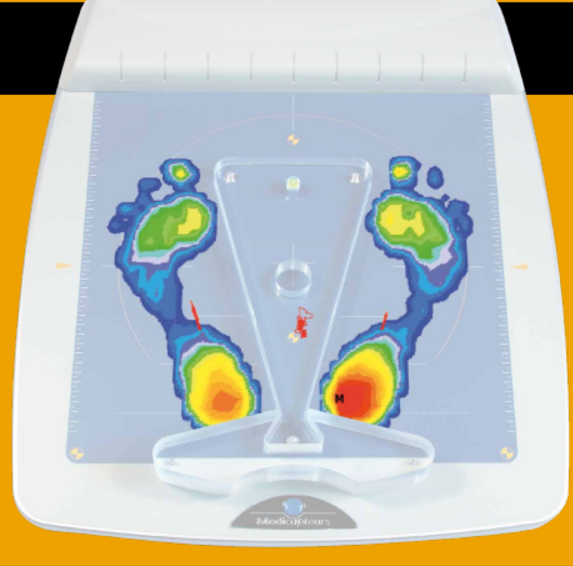
\includegraphics[height=5cm]{images/analyse_marche/Fusyo_1.png}
      \caption{Plateforme d'analyse Fusyo}\label{fig:Fusyo_1}
    \end{subfigure}\\
    \begin{subfigure}[b]{0.45\textwidth}
        \hspace{-4.5cm}
        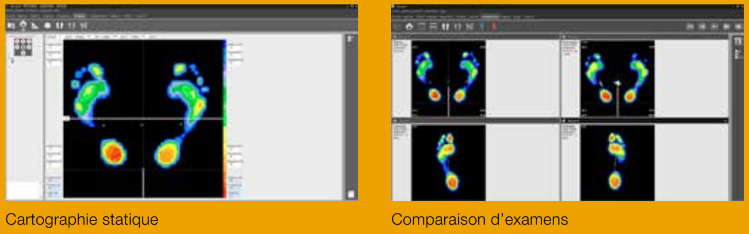
\includegraphics[height=5cm]{images/analyse_marche/Fusyo_2.png}
        \caption{Outils de comparaison des cartographies statiques}\label{fig:Fusyo_2}
    \end{subfigure}\\
    \begin{subfigure}[b]{0.45\textwidth}
        \hspace{-5cm}
        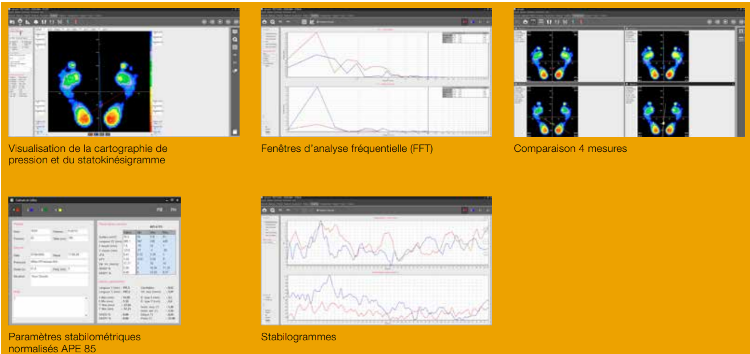
\includegraphics[height=8cm]{images/analyse_marche/Fusyo_4.png}
        \caption{Outils de visualisations des données stabilométriques}\label{fig:Fusyo_4}
    \end{subfigure}
\end{figure}

\subsection{FOOTWORK PRO}

FootWork Pro est conçu pour les analyses statiques et dynamiques. 
Il inclut des fonctionnalités avancées telles que centre des pressions, 
pression maxi de chaque pied, répartition avant et arrière, droite et gauche. 
Projection du centre de gravité, zone d’études et film de la statique.  
Possibilité de paramétrer la durée, la fréquence et le pourcentage des points.
Il est compatible avec les ordinateurs Windows, cette plateforme d’analyse est simple à intégrer 
dans des environnements de travail classiques.
Il permet l'édition des comptes rendus et permet la possibilité d’envoi par mail 
des analyses avec création des fichiers patients.

FootWork Pro est conçu pour les analyses statiques. 
Cette plateforme d’analyse a comme fonctionnalités:

\begin{itemize}
    \item \textbf Fichier patients
    \item \textbf Analyse statique : centre des pressions, pression maxi de chaque pied, répartition avant et arrière, droite et gauche. Projection du centre de gravité, zone d’études et film de la statique.
    \item \textbf Stabilométrie : ellipses et dimensions des centres de poussée. Oscillation et pourcentage en surface et en temps : plan frontal, sagittal. Possibilité de paramétrer la durée, la fréquence et le pourcentage des points. Analyse unipodale.
    \item \textbf Analyse dynamique : pas multiples avec reconnaissance automatique pied droit / pied gauche. Pressions moyennes et maxi, durée d’appui et intégrale pression / temps. Zones d’études : précise les zones de travail du pied. Automatiques, intelligentes, manuelles et médio-latérale. Analyse des 3 temps du pas avec superposition d'une référence. Vidéo 3D.
    \item \textbf Compatible PC Windows uniquement.
    \item \textbf Editions des comptes rendus et possibilité d’envoi par mail des analyses.
    \item \textbf Inclus 3 ans de contrat d’assistance et de mise à jour
\end{itemize}

\begin{figure}[H]
    \centering
    \begin{subfigure}[b]{0.45\textwidth}
      \centering
        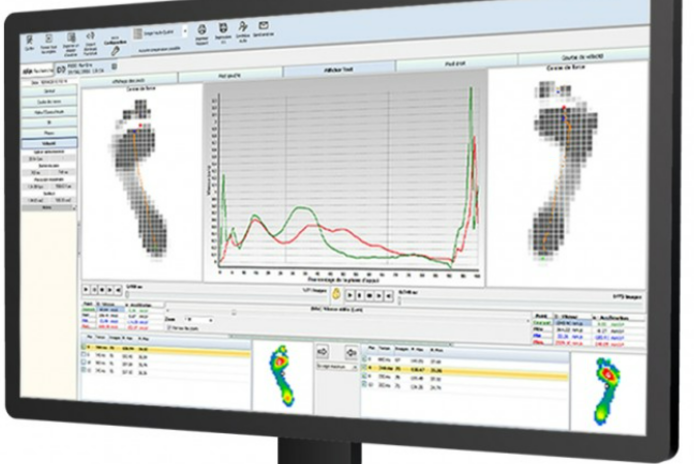
\includegraphics[height=5cm]{images/analyse_marche/Footwork_pro.png}
        \caption{Outil de visualisation des données posturographiques FootWork}\label{fig:Footwork_pro}
    \end{subfigure}
    \begin{subfigure}[b]{0.5\textwidth}
        \centering
        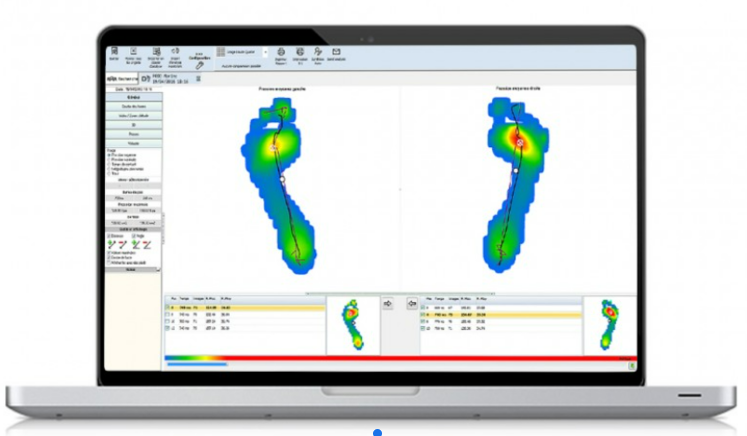
\includegraphics[height=5cm]{images/analyse_marche/Footwork_pro_1.png}
        \caption{Outil de visualisation 3D des centre de pression Footwork}\label{fig:Footwork_pro1}
    \end{subfigure}
    \begin{subfigure}[b]{0.5\textwidth}
        \centering  
        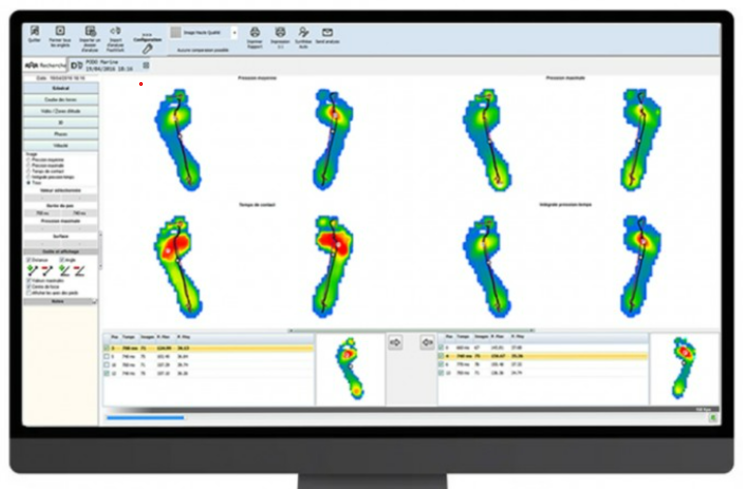
\includegraphics[height=5cm]{images/analyse_marche/Footwork_pro_2.png}
        \caption{Outil de comparaison des models 3D Footwork}\label{fig:Footwork_pro2}
    \end{subfigure}
\end{figure}


\subsection{Win-pod}

WinPod est une solution intuitive destinée aux analyses posturales simples 
et qualitatives. Il permet de personnaliser les rapports en y ajoutant photos, 
commentaires et modèles prédéfinis. En temps réel, il génère des cartographies et
 suit l’évolution des centres de pression. Cependant, WinPod est limité en termes 
 d’analyses avancées et convient mieux aux besoins cliniques de base ou aux bilans 
 qualitatifs qu’aux études approfondies.

 WinPod est une solution intuitive destinée aux analyses posturales 
 simples et qualitatives. Cette plateforme d’analyse a comme fonctionnalités:

\begin{itemize}
    \item \textbf Cartographie statique avec calcul par zone
    \item \textbf Multitude de visualisations (thermographique, isopression,3D…)
    \item \textbf Analyse numérique et graphique des paramètres de stabilométrie
    \item \textbf Evolution des cartographies et des centres de pression
    \item \textbf Quotient de Romberg
    \item \textbf Visualisation temps réel
    \item \textbf Archivage de tout type de documents électronique à la fiche d’examen clinique
    \item \textbf Rapport personnalisable : insertion de photos, ajout, de commentaires
    \item \textbf Exportation au format PDF
    \item \textbf Intégration du foot posture index FPI (Normalisation internationale du pied)
    \item \textbf Calcul du CPEI (Centre of Pressure Foot Index)
    \item \textbf Impression à l'échelle 1/1
    \item \textbf Comparaison d’examens
    \item \textbf File d’impression

\end{itemize}

 \begin{figure}[H]
    \centering
    \begin{subfigure}[b]{0.45\textwidth}
      \centering
        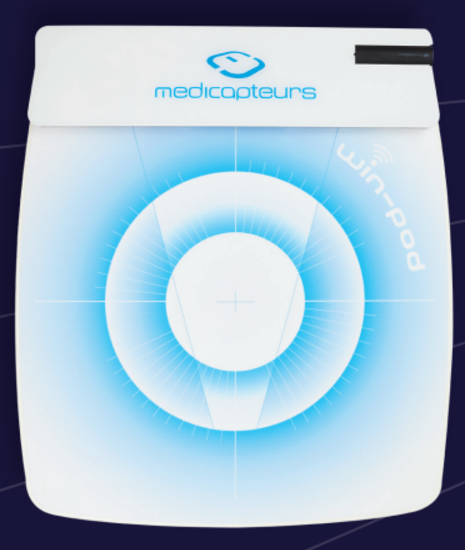
\includegraphics[height=5cm]{images/analyse_marche/WinPod.png}
        \caption{Plateforme stabilométriques Win-pod}\label{fig:WinPod}
    \end{subfigure}
    \begin{subfigure}[b]{0.5\textwidth}
        \centering
        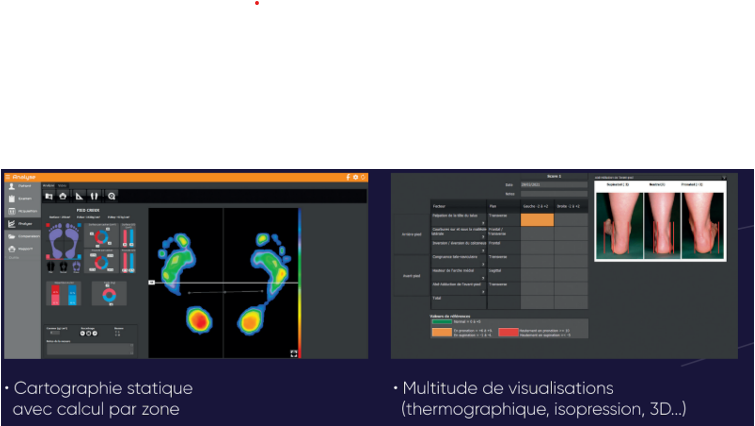
\includegraphics[height=5cm]{images/analyse_marche/WinPod1.png}
        \caption{Outil de comparaison de données 3D et de photos Win-pod }\label{fig:WinPod1}
    \end{subfigure} 
    \begin{subfigure}[b]{0.5\textwidth}
        \hspace{-2.5cm} 
        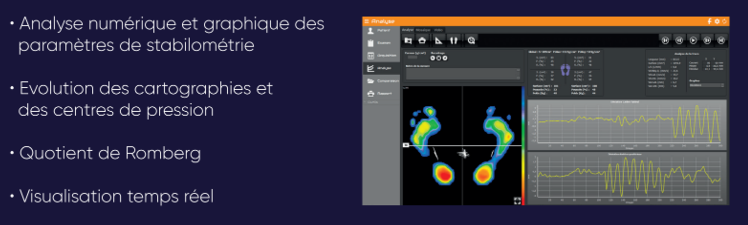
\includegraphics[height=4cm]{images/analyse_marche/WinPod2.png}
        \caption{Outil de visualisation des siganux posturographiques}\label{fig:WinPod2}
    \end{subfigure}
\end{figure}

\subsection{SabotSoft}

SabotSoft est une solution avancée pour les analyses détaillées des oscillations 
corporelles et des déséquilibres posturaux. Il intègre des modèles complexes, 
tels que les vecteurs de vitesse, ou les spectres croisés, souvent utilisés pour 
identifier des pathologies neurologiques spécifiques. Son interface, bien que avancée,
requiert une expertise technique pour être exploitée au maximum. 
Les graphiques et représentations visuelles qu’il propose sont d’une grande précision,
facilitant l’interprétation des données pour des experts en biomécanique ou 
neurologie.

SabotSoft est une solution avancée pour les analyses détaillées 
des oscillations corporelles et des déséquilibres posturaux. 
Cette plateforme d’analyse a comme fonctionnalités : 

\begin{itemize}
    \item \textbf {Statokinésigrammes et ellipses de confiance} 
    \item \textbf {Centre de pressions et centre de masse} 
    \item \textbf {Contrôle et sur-contrôle des oscillations (densité spectrale d’interaction)}
    \item \textbf {Vectogramme du centre de pressions et du centre de masses}
    \begin{itemize}
        \item Distribution des vecteurs vitesse par secteur autour de l’origine.
        \item Détection des singularités et limites du modèle du pendule inversé mono-articulé.
        \item Révélation des blocages fonctionnels (par exemple, non-alignement des axes de cheville) ou des dysfonctions (ex. : jambe courte).
    \end{itemize} 
    \item \textbf{Spectre des forces verticales :}
    \begin{itemize}
    \item Analyse par FFT de la résultante des forces verticales $Z(t)$.
    \item Identification de mouvements verticaux de haute fréquence et de trémors pathologiques.
    \end{itemize}
    \item \textbf{Diagramme des asymétries :}
    \begin{itemize}
    \item Visualisation des asymétries des placements moyens du centre de pressions (CdP).
    \item Comparaison avec une référence normative basée sur une population témoin.
    \item Identification des écarts de position et de direction, illustrés par des vecteurs.
    \item Différences entre les enregistrements en condition yeux ouverts et yeux fermés.
    \end{itemize}
    \item \textbf{Ondelette :}
    \begin{itemize}
        \item Représentation temps-fréquence du signal stabilométrique à l’aide d’ondelettes.
    \item Analyse tridimensionnelle (temps-fréquence-intensité) ou plane (par code couleur).
    \end{itemize}
\end{itemize}



\begin{figure}[H]
    \centering
    \begin{subfigure}[b]{0.45\textwidth}
      \centering
        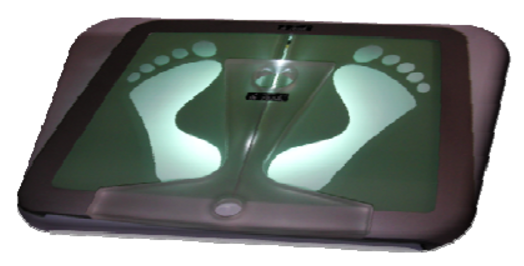
\includegraphics[height=3.5cm]{images/analyse_marche/SabotSoft1.png}
        \caption{Plateforme stabilométriques SobotSoft}\label{fig:sabotsoft1}
    \end{subfigure}
    \begin{subfigure}[b]{0.5\textwidth}
        \centering
        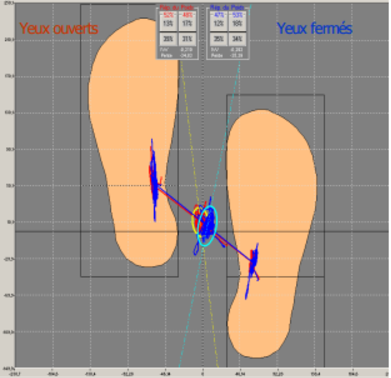
\includegraphics[height=4cm]{images/analyse_marche/SabotSoft2.png}
        \caption{Outil de visualisation de centre de pression yeux ouverts et fermés}\label{fig:SabotSoft23}
    \end{subfigure}\\
    \begin{subfigure}[b]{0.5\textwidth}
        \hspace{-1.5cm} 
        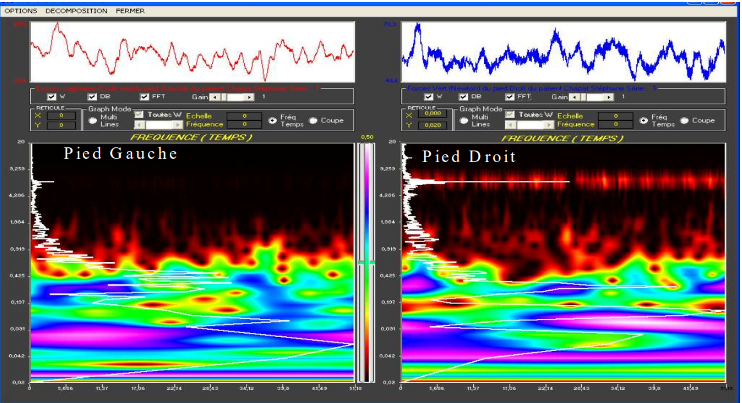
\includegraphics[height=6cm]{images/analyse_marche/SabotSoft5.png}
        \caption{Outil d'analyse de x et y dans le domaine temporel}\label{fig:SabotSoft5}
    \end{subfigure}
\end{figure}
